\documentclass[article]{jss}

%% -- LaTeX packages and custom commands ---------------------------------------

\usepackage{orcidlink,thumbpdf,lmodern}
\usepackage{amsmath,amssymb,bm,booktabs,framed}

\newcommand{\class}[1]{`\code{#1}'}
\newcommand{\fct}[1]{\code{#1()}}

%% For Sweave-based articles about R packages:


%% -- Article metainformation (author, title, ...) -----------------------------

\author{Ridson Al Farizal P.~\orcidlink{0009-0007-8280-9944}\\Politeknik Statistika STIS
   \And Azka Ubaidillah\\Politeknik Statistika STIS}
\Plainauthor{Ridson Al Farizal P., Azka Ubaidillah}

\title{\pkg{fastsae}: High-Performance Frequentist and Bayesian Small Area Estimation in \proglang{R}}
\Plaintitle{fastsae: High-Performance Frequentist and Bayesian Small Area Estimation in R}
\Shorttitle{\pkg{fastsae}: High-Performance Small Area Estimation in \proglang{R}}

\Abstract{
  Small area estimation (SAE) plays a pivotal operational role in official statistics, enabling the production of reliable disaggregated socioeconomic, health, and demographic indicators when domain-specific sample sizes are small or zero. However, practitioners in national statistical offices (NSOs) face a dual computational barrier: frequentist spatial and spatio-temporal models with bootstrap mean squared error (MSE) estimation are hindered by severe computational bottlenecks in interpreted languages, while non-Gaussian indicators (such as rates, skewed expenditures, and counts) traditionally require computationally demanding Markov chain Monte Carlo (MCMC) algorithms that impede routine production. We introduce \pkg{fastsae}, an \proglang{R} package engineered for high-performance frequentist and Bayesian small area estimation. On the frequentist side, \pkg{fastsae} implements optimized \proglang{C++17} routines via \pkg{RcppArmadillo} paired with OpenMP multi-threading, accelerating the classical Fay-Herriot, spatial Fay-Herriot, spatio-temporal Fay-Herriot, and unit-level Battese-Harter-Fuller models alongside their analytical and bootstrap MSE estimators. On the Bayesian side, \pkg{fastsae} provides a unified empirical best prediction (EBP) interface powered by Integrated Nested Laplace Approximations (\pkg{INLA}) across six distribution families (Gaussian, Beta, Gamma, Binomial, Poisson, Negative Binomial). Crucially, \pkg{fastsae} introduces exact survey dispersion mappings that respect design-based direct sampling variances and accommodates modern spatial priors (BYM, scaled BYM2, Leroux CAR, and SLM). The package also features a comprehensive diagnostic engine, automated \pkg{ggplot2} visualizations, and configurable simulation generators. Extensive benchmarks demonstrate multi-fold computational speedups over existing packages without loss of inferential precision.
}

\Keywords{small area estimation, Fay-Herriot, empirical best prediction, INLA, OpenMP, Rcpp, spatial statistics, \proglang{R}}
\Plainkeywords{small area estimation, Fay-Herriot, empirical best prediction, INLA, OpenMP, Rcpp, spatial statistics, R}

\Address{
  Ridson Al Farizal P.\\
  Department of Computational Statistics\\
  Politeknik Statistika STIS\\
  Jl. Otto Iskandardinata No. 64C\\
  Jakarta Timur 13330, Indonesia\\
  E-mail: \email{ridson@stis.ac.id}\\
  \emph{and}\\
  Azka Ubaidillah\\
  Department of Statistics\\
  Politeknik Statistika STIS\\
  Jl. Otto Iskandardinata No. 64C\\
  Jakarta Timur 13330, Indonesia\\
  E-mail: \email{azka@stis.ac.id}
}

\usepackage{Sweave}
\begin{document}

%% -- Introduction -------------------------------------------------------------

\section{Introduction} \label{sec:intro}

In modern evidence-based policymaking, the demand for reliable statistical indicators at highly disaggregated geographic and administrative levels---such as municipalities, districts, and health administrative zones---has grown exponentially. High-resolution local data are indispensable for monitoring the United Nations Sustainable Development Goals (SDGs), allocating targeted intergovernmental fiscal equalization funds, identifying localized poverty pockets, and tailoring community health interventions \citep{rao2015small, pfeffermann2013new}. However, national sample surveys conducted by National Statistical Offices (NSOs)---such as the American Community Survey (ACS) in the United States, the European Union Statistics on Income and Living Conditions (EU-SILC), and the National Socioeconomic Survey (Susenas) in Indonesia---are typically powered to yield dependable direct estimators only at macroscopic national or regional domains. When sample survey data are partitioned into smaller sub-populations, the domain-specific sample sizes become inevitably small, and certain domains may remain entirely unsampled. Consequently, direct survey estimators suffer from excessively large standard errors, unacceptable coefficients of variation, and extreme volatility, rendering them inadequate for micro-level policy formulation and regional resource planning \citep{burgard2020computational, pratesi2016analysis}.

To address the inferential deficiencies of direct survey estimators, small area estimation (SAE) methodologies have emerged as an essential branch of modern survey statistics. The fundamental principle underpinning SAE is to ``borrow strength'' across related domains and time periods through explicit linking models that incorporate auxiliary information from recent censuses, administrative registers, or earth observation data \citep{rao2015small}. Within the broad taxonomy of area-level models, the classical Fay-Herriot (FH) model \citep{fay1979estimates} remains the cornerstone of official statistics production due to its conceptual elegance, its minimal data requirements, and its ability to respect survey design variances without requiring access to confidential individual-level microdata.

Nevertheless, standard area-level models assume that domain-specific random effects are independent and identically distributed. In spatial phenomena, this independence assumption is routinely violated because geographical units that are spatially contiguous frequently exhibit substantial spatial autocorrelation, in accordance with Tobler's First Law of Geography \citep{tobler1970computer}. To account for spatial dependence, \citet{petrucci2006small} and \citet{pratesi2008small} introduced the Spatial Fay-Herriot (SFH) model, which embeds a Simultaneous Autoregressive (SAR) error process into the area random effects via an exogenously specified spatial proximity matrix. \citet{marhuenda2013small} further generalized this framework to the Spatio-Temporal Fay-Herriot (ST-FH) model by simultaneously modeling spatial SAR structures alongside first-order autoregressive (AR(1)) temporal dynamics across panel observation windows. Similarly, when unit-level microdata are available, the nested error regression model of \citet{battese1988error} (BHF) provides empirical best linear unbiased predictors (EBLUP) at the sub-domain level. While these models represent significant methodological milestones, their inferential procedures---namely variance component estimation via Restricted Maximum Likelihood (REML) and Mean Squared Error (MSE) estimation via analytical approximations or bootstrap resampling \citep{gonzalez2008bootstrap}---require repeated high-dimensional matrix inversions and iterative Fisher-scoring steps that become computationally prohibitive on large geographical scales.

A further critical challenge in small area estimation arises when target indicators deviate fundamentally from the Gaussian assumption. Real-world policy indicators frequently exhibit structural distributional boundaries that linear models fail to accommodate. For example, welfare indicators representing rates or proportions---such as poverty headcounts, unemployment rates, illiteracy, and child stunting prevalence---are strictly bounded within the unit interval $(0, 1)$. Applying conventional Gaussian linear models to such bounded endpoints often yields nonsensical out-of-bounds estimates ($< 0$ or $> 1$) and distorts variance structures \citep{janicki2020properties, denicolo2022tipsae}. While ad-hoc transformations (such as the logit or arcsine square-root) are common in practice, transforming model estimates back to the original measurement scale induces severe, non-linear back-transformation biases \citep{slud2006mean}. Similarly, monetary welfare metrics such as household per capita expenditures, income distribution parameters, and poverty gap indices exhibit pronounced right-skewness where the variance scales quadratically with the mean, naturally adhering to a Gamma distribution \citep{ghosh2004small, fabrizi2011hierarchical}. Furthermore, discrete demographic events, including localized disease counts or maternal mortality occurrences, follow Poisson or overdispersed Negative Binomial processes governed by area-specific population exposures \citep{boubeta2016empirical, boubeta2017poisson}.

Under non-Gaussian likelihoods, the classical linear theory of EBLUP is inapplicable, necessitating Generalized Linear Mixed Models (GLMM) and Empirical Best Prediction (EBP) within a Hierarchical Bayesian (HB) formulation \citep{rao2015small}. Traditionally, HB models are estimated via Markov Chain Monte Carlo (MCMC) algorithms, including Gibbs sampling and Hamiltonian Monte Carlo (HMC) implemented in generic engines such as \pkg{JAGS} or \pkg{Stan} \citep{gelman2013bayesian}. However, MCMC sampling introduces severe computational bottlenecks: generating tens of thousands of dependent iterations requires substantial runtime (often several hours for national grids), mandates laborious convergence diagnostics such as Gelman-Rubin $\hat{R}$ statistics and trace plot inspections, and frequently suffers from divergent transitions when complex spatial priors---such as the Intrinsic Conditional Autoregressive (ICAR) model of \citet{besag1991bayesian} or the Leroux CAR model \citep{leroux2000estimation}---are specified over sparse graph topologies \citep{simpson2017penalising}. These operational barriers severely impede the automated, reproducible implementation of SAE in official production environments. To circumvent the computational friction of MCMC, \citet{rue2009approximate} introduced Integrated Nested Laplace Approximations (INLA) for the class of Latent Gaussian Models (LGMs). Instead of relying on stochastic sampling simulations, INLA exploits the conditional independence properties of Gaussian Markov Random Fields (GMRF) and utilizes low-order Taylor expansions with sparse matrix algebra to compute deterministic, highly accurate approximations of marginal posterior distributions in seconds rather than hours \citep{rue2017bayesian, gomez2020bayesian}. While INLA has revolutionized spatial epidemiology and environmental statistics \citep{bivand2015spatial}, its systematic adoption within small area estimation has remained fragmented due to the lack of specialized software interfaces capable of automatically mapping direct design-based sampling variances, sample sizes, and exposure offsets into corresponding likelihood dispersion parameters.

An examination of the current \proglang{R} software ecosystem reveals that existing small area estimation packages are specialized yet compartmentalized. The venerable \pkg{sae} package \citep{molina2015sae} provides classical FH and spatial SFH estimators, but its computational engine is implemented in pure interpreted \proglang{R}, lacks multi-threading, is restricted to Gaussian responses, and exhibits long runtimes for bootstrap MSE estimation. The \pkg{emdi} package \citep{kreutzmann2019emdi} offers an elegant interface and visualization tools for unit- and area-level models, but lacks native spatio-temporal AR(1) dynamics and non-Gaussian spatial Bayesian likelihoods. Specialized packages such as \pkg{tipsae} \citep{denicolo2022tipsae} implement Beta regression for area-level proportions using Stan, but are tied to MCMC runtimes that scale poorly for complex spatial adjacency graphs. Meanwhile, general Bayesian SAE toolkits (e.g., \pkg{saeHB}) rely on JAGS, inheriting the convergence inspection burdens and computational delays inherent to MCMC. To date, no single computational framework unites high-performance compiled frequentist engines with fast, non-Gaussian spatial Bayesian EBP approximations.

To bridge this methodological and computational divide, we introduce the \proglang{R} package \pkg{fastsae}. Designed as an ultra-fast, comprehensive, and scalable computational environment for small area estimation, \pkg{fastsae} addresses both frequentist and Bayesian paradigms through several major architectural innovations. On the frequentist side, \pkg{fastsae} implements optimized \proglang{C++17} computational routines via \pkg{Rcpp} \citep{eddelbuettel2011rcpp} and \pkg{RcppArmadillo} \citep{eddelbuettel2014rcpparmadillo} paired with OpenMP multi-threading for the standard Fay-Herriot (\code{eblup\_fh()}), Spatial Fay-Herriot (\code{eblup\_sfh()}), Spatio-Temporal Fay-Herriot (\code{eblup\_stfh()}), and unit-level Battese-Harter-Fuller (\code{eblup\_bhf()}) models, delivering orders-of-magnitude speedups for analytical and parametric or non-parametric bootstrap MSE estimation. On the Bayesian side, \pkg{fastsae} provides the unified \code{ebp\_area()} interface powered by \pkg{R-INLA}, encompassing six distinct likelihood families: Gaussian, Beta, Gamma, Binomial, Poisson, and Negative Binomial. Crucially, the package embeds exact, distribution-specific dispersion mappings that respect survey sampling uncertainty: observational precision scaling $\tau_i = 1/D_i$ for Gaussian responses, the \citet{janicki2020properties} direct dispersion formula $\phi_i = \max(y_i(1-y_i)/D_i - 1, 1)$ for Beta proportions, direct coefficient of variation scaling $s_i = y_i^2/D_i = 1/CV_i^2$ for Gamma responses, and automated trial or exposure scaling for count models. Furthermore, \pkg{fastsae} supports modern spatial priors including the classic Besag-York-Molli\'e (BYM) model, the scaled BYM2 specification with Penalized Complexity (PC) priors \citep{simpson2017penalising}, the Leroux CAR specification with exact precision structure $C = I - R$, and Simultaneous Autoregressive Spatial Lag Models (SLM) with spectral eigenvalue bounds.

Complementing its modeling engines, \pkg{fastsae} provides an integrated suite of post-estimation diagnostic, visualization, and simulation tools. A universal diagnostic function, \code{diagnose()}, computes Bayesian information criteria (DIC, WAIC, marginal log-likelihood), leave-one-out predictive cross-validation metrics (Conditional Predictive Ordinate, CPO; Probability Integral Transform, PIT), and simulation evaluation statistics (Relative Root Mean Squared Error, Relative Bias, Mean Absolute Difference). Automated graphical diagnostics via \code{autoplot()} allow practitioners to visually inspect shrinkages, residual distributions, spatial random fields, and precision profiles using standard \pkg{ggplot2} graphics \citep{wickham2016ggplot2}. For empirical validation and reproducible research, the package includes multi-distribution benchmark datasets (\code{sim\_area} and \code{sim\_panel}) alongside configurable data generators (\code{sim\_area\_data()} and \code{sim\_series\_data()}) that allow researchers to simulate cross-sectional and longitudinal small area survey datasets under complex spatial and temporal autocorrelation structures.

The remainder of this article is structured as follows. Section~\ref{sec:methods} formalizes the statistical methodologies, covering the frequentist spatial and spatio-temporal EBLUP specifications alongside the Bayesian non-Gaussian INLA formulations. Section~\ref{sec:design} details the software architecture, design principles, and user-facing functions of \pkg{fastsae}. Section~\ref{sec:simulations} presents extensive simulation studies evaluating point estimation accuracy, inferential calibration, and computational speedups relative to established benchmarks (\pkg{sae} and \pkg{tipsae}). Section~\ref{sec:applications} demonstrates the practical utility of \pkg{fastsae} through empirical applications to official socioeconomic indicators. Section~\ref{sec:summary} concludes with a summary of contributions and an outline of ongoing extensions.

%% -- Methodological Framework -------------------------------------------------

\section{Methodological framework} \label{sec:methods}

\subsection{Frequentist small area models} \label{sec:methods_freq}

\subsubsection{Classical Fay-Herriot model}
Let $m$ denote the total number of small areas indexed by $i = 1, \dots, m$. The classical area-level model of \citet{fay1979estimates} consists of two stages: a sampling model and a linking model. The sampling model assumes that the design-based direct estimator $y_i$ is conditionally unbiased for the true area parameter $\theta_i$, with known design variance $D_i = \mathrm{Var}_p(y_i \mid \theta_i)$:
%
\begin{equation} \label{eq:fh_sampling}
y_i = \theta_i + e_i, \quad e_i \overset{\mathrm{ind}}{\sim} \mathcal{N}(0, D_i).
\end{equation}
%
The linking model relates the latent parameter $\theta_i$ to a $p \times 1$ vector of area-level auxiliary covariates $\bm{x}_i$ through a linear regression:
%
\begin{equation} \label{eq:fh_linking}
\theta_i = \bm{x}_i^\top \bm{\beta} + u_i, \quad u_i \overset{\mathrm{iid}}{\sim} \mathcal{N}(0, \sigma_u^2),
\end{equation}
%
where $\bm{\beta}$ is the vector of fixed regression coefficients, and $u_i$ is an area-specific random effect assumed independent of the sampling error $e_i$. Combining (\ref{eq:fh_sampling}) and (\ref{eq:fh_linking}) yields the linear mixed model $y_i = \bm{x}_i^\top \bm{\beta} + u_i + e_i$. Under known $\sigma_u^2$, the best linear unbiased predictor (BLUP) of $\theta_i$ is a precision-weighted convex combination:
%
\begin{equation} \label{eq:fh_blup}
\tilde{\theta}_i = \gamma_i y_i + (1 - \gamma_i) \bm{x}_i^\top \tilde{\bm{\beta}},
\end{equation}
%
where $\gamma_i = \sigma_u^2 / (\sigma_u^2 + D_i)$ is the shrinkage factor, and $\tilde{\bm{\beta}} = (\bm{X}^\top \bm{V}^{-1} \bm{X})^{-1} \bm{X}^\top \bm{V}^{-1} \bm{y}$ is the generalized least squares (GLS) estimator with diagonal covariance matrix $\bm{V} = \mathrm{diag}(\sigma_u^2 + D_1, \dots, \sigma_u^2 + D_m)$. When $\sigma_u^2$ is replaced by an empirical estimator $\hat{\sigma}_u^2$ obtained via REML or ML, (\ref{eq:fh_blup}) becomes the Empirical BLUP (EBLUP), $\hat{\theta}_i$. Its mean squared error is evaluated using the second-order accurate analytical approximation of \citet{prasad1990estimation}:
%
\begin{equation} \label{eq:fh_mse}
\mathrm{MSE}(\hat{\theta}_i) \approx g_{1i}(\hat{\sigma}_u^2) + g_{2i}(\hat{\sigma}_u^2) + 2 g_{3i}(\hat{\sigma}_u^2),
\end{equation}
%
where $g_{1i} = \gamma_i D_i$, $g_{2i} = (1 - \gamma_i)^2 \bm{x}_i^\top (\bm{X}^\top \bm{V}^{-1} \bm{X})^{-1} \bm{x}_i$, and $g_{3i} = D_i^2 (\sigma_u^2 + D_i)^{-3} \overline{\mathrm{Var}}(\hat{\sigma}_u^2)$ accounts for the variability in estimating the variance component.

\subsubsection{Spatial Fay-Herriot model}
To incorporate spatial correlation across geographic domains, \citet{petrucci2006small} and \citet{pratesi2008small} modeled the area random effects $\bm{u} = (u_1, \dots, u_m)^\top$ via a first-order Simultaneous Autoregressive (SAR) process:
%
\begin{equation} \label{eq:sfh_sar}
\bm{u} = \rho \bm{W} \bm{u} + \bm{\epsilon}, \quad \bm{\epsilon} \sim \mathcal{N}_m(\bm{0}, \sigma_1^2 \bm{I}_m),
\end{equation}
%
where $\rho$ is the spatial autoregressive parameter, $\bm{W}$ is an $m \times m$ row-standardized spatial proximity matrix, and $\bm{\epsilon}$ is an innovation vector. Assuming $(\bm{I}_m - \rho \bm{W})$ is invertible, $\bm{u} = (\bm{I}_m - \rho \bm{W})^{-1} \bm{\epsilon}$, resulting in $\mathrm{Var}(\bm{u}) = \bm{G}(\sigma_1^2, \rho) = \sigma_1^2 [(\bm{I}_m - \rho \bm{W})^\top (\bm{I}_m - \rho \bm{W})]^{-1}$. The marginal covariance of $\bm{y}$ is $\bm{V}(\sigma_1^2, \rho) = \bm{G}(\sigma_1^2, \rho) + \bm{D}$, where $\bm{D} = \mathrm{diag}(D_1, \dots, D_m)$. 

The spatial EBLUP of $\bm{\theta} = \bm{X} \bm{\beta} + \bm{u}$ takes the matrix form:
%
\begin{equation} \label{eq:sfh_eblup}
\hat{\bm{\theta}} = \bm{X} \hat{\bm{\beta}} + \hat{\bm{G}} \hat{\bm{V}}^{-1} (\bm{y} - \bm{X} \hat{\bm{\beta}}),
\end{equation}
%
where $\hat{\bm{\beta}} = (\bm{X}^\top \hat{\bm{V}}^{-1} \bm{X})^{-1} \bm{X}^\top \hat{\bm{V}}^{-1} \bm{y}$. Variance components $(\sigma_1^2, \rho)$ are estimated via profile REML over the valid parameter space $\rho \in (\lambda_{\min}^{-1}, \lambda_{\max}^{-1})$, where $\lambda_{\min}$ and $\lambda_{\max}$ represent the minimum and maximum eigenvalues of $\bm{W}$. For MSE estimation, \pkg{fastsae} implements both the analytical Singh-Shukla-Kundu approximation and the parametric bootstrap procedure of \citet{gonzalez2008bootstrap}.

\subsubsection{Spatio-temporal Fay-Herriot model}
When small area data are collected across multiple time periods $t = 1, \dots, T$, borrowing strength across both space and time yields substantial efficiency gains. The spatio-temporal Fay-Herriot model of \citet{marhuenda2013small} specifies:
%
\begin{equation} \label{eq:stfh_model}
y_{it} = \bm{x}_{it}^\top \bm{\beta} + u_{1,it} + u_{2,it} + e_{it},
\end{equation}
%
where $\bm{u}_{1,t} = (u_{1,1t}, \dots, u_{1,mt})^\top$ follows a spatial SAR process $\bm{u}_{1,t} = \rho_1 \bm{W} \bm{u}_{1,t} + \bm{\epsilon}_{1,t}$ with $\bm{\epsilon}_{1,t} \sim \mathcal{N}_m(\bm{0}, \sigma_1^2 \bm{I}_m)$, and $u_{2,it}$ follows an area-specific temporal AR(1) process $u_{2,it} = \rho_2 u_{2,i,t-1} + \epsilon_{2,it}$ with $|\rho_2| < 1$ and $\epsilon_{2,it} \sim \mathcal{N}(0, \sigma_2^2)$. In \pkg{fastsae}, the block-structured covariance matrix $\bm{V}(\bm{\theta}_v)$ is assembled and inverted using optimized Kronecker product routines, enabling rapid REML parameter convergence and parallelized bootstrap MSE estimation.

\subsubsection{Unit-level Battese-Harter-Fuller model}
When sample microdata are accessible alongside population auxiliary totals, \pkg{fastsae} provides the nested error regression model of \citet{battese1988error}:
%
\begin{equation} \label{eq:bhf_model}
y_{dj} = \bm{x}_{dj}^\top \bm{\beta} + u_d + e_{dj}, \quad d = 1, \dots, D, \quad j = 1, \dots, n_d,
\end{equation}
%
where $u_d \overset{\mathrm{iid}}{\sim} \mathcal{N}(0, \sigma_u^2)$ and $e_{dj} \overset{\mathrm{iid}}{\sim} \mathcal{N}(0, \sigma_e^2)$. For an in-sample domain $d$ with population size $N_d$ and population covariate mean vector $\bar{\bm{X}}_d$, the EBLUP is given by:
%
\begin{equation} \label{eq:bhf_eblup}
\hat{\bar{Y}}_d = f_d \bar{y}_d + (1 - f_d) \left( \bar{\bm{X}}_{d, r}^\top \hat{\bm{\beta}} + \hat{\gamma}_d (\bar{y}_d - \bar{\bm{x}}_d^\top \hat{\bm{\beta}}) \right),
\end{equation}
%
where $f_d = n_d / N_d$ is the sampling fraction, $\hat{\gamma}_d = \hat{\sigma}_u^2 / (\hat{\sigma}_u^2 + \hat{\sigma}_e^2 / n_d)$, and $\bar{\bm{X}}_{d, r}$ is the mean of non-sampled units. For an unsampled domain ($n_d = 0$), the synthetic predictor is $\hat{\bar{Y}}_d = \bar{\bm{X}}_d^\top \hat{\bm{\beta}}$.

\subsection{Bayesian non-Gaussian hierarchical EBP via INLA} \label{sec:methods_inla}

\subsubsection{Latent Gaussian models}
For non-Gaussian indicators, \pkg{fastsae} formulates the small area problem within the Latent Gaussian Model (LGM) framework \citep{rue2009approximate}. Let $y_i$ be an observed direct response for area $i$. The likelihood is assumed conditionally independent given the latent predictor $\eta_i$ and hyperparameters $\bm{\theta}$:
%
\begin{equation} \label{eq:lgm_likelihood}
y_i \mid \eta_i, \bm{\theta} \sim \pi(y_i \mid \eta_i, \bm{\theta}).
\end{equation}
%
The linear predictor $\eta_i = g(\mu_i)$ incorporates fixed auxiliary effects and structured/unstructured random components:
%
\begin{equation} \label{eq:lgm_predictor}
\eta_i = \bm{x}_i^\top \bm{\beta} + u_i + v_i,
\end{equation}
%
where $\bm{\beta} \sim \mathcal{N}(\bm{0}, \sigma_\beta^2 \bm{I}_p)$, $v_i \overset{\mathrm{iid}}{\sim} \mathcal{N}(0, \tau_v^{-1})$ is an unstructured IID effect, and $\bm{u} = (u_1, \dots, u_m)^\top$ represents a spatial Gaussian Markov Random Field (GMRF) with precision matrix $\bm{Q}(\bm{\theta}_s)$. The joint latent vector $\bm{\psi} = (\bm{\beta}^\top, \bm{u}^\top, \bm{v}^\top)^\top$ follows a high-dimensional multivariate Gaussian distribution $\bm{\psi} \sim \mathcal{N}(\bm{0}, \bm{Q}^{-1})$. INLA approximates the marginal posteriors $\pi(\psi_j \mid \bm{y})$ and $\pi(\theta_k \mid \bm{y})$ deterministically using Laplace approximations and numerical integration over a low-dimensional grid of $\bm{\theta}$.

\subsubsection{Exact survey dispersion and variance matching}
A central innovation in \pkg{fastsae} is the automatic, exact mapping between design-based survey variance estimates and INLA likelihood dispersion parameters across six distribution families:
%
\begin{enumerate}
  \item \textbf{Gaussian}: The observational precision is fixed directly to the inverse design variance:
  \begin{equation}
  \tau_i = \frac{1}{D_i}.
  \end{equation}
  \item \textbf{Beta}: For proportions $y_i \in (0, 1)$ with logit link $\mathrm{logit}(\mu_i) = \eta_i$, the Beta density is parameterized by mean $\mu_i$ and precision $\phi_i$ such that $\mathrm{Var}(y_i \mid \mu_i, \phi_i) = \mu_i(1 - \mu_i) / (1 + \phi_i)$. Equating this model-based variance to the direct design variance $D_i$ yields the \citet{janicki2020properties} dispersion parameter:
  \begin{equation} \label{eq:beta_dispersion}
  \phi_i = \max\left( \frac{y_i (1 - y_i)}{D_i} - 1, \, 1 \right).
  \end{equation}
  In \pkg{fastsae}, $\phi_i$ is injected area-by-area into \pkg{R-INLA} via the \code{scale} argument, with the global precision hyperparameter fixed to unity ($\theta = 0$), ensuring exact preservation of area-specific design variances.
  \item \textbf{Gamma}: For strictly positive, right-skewed monetary indicators $y_i > 0$ with log link $\log(\mu_i) = \eta_i$, the Gamma variance is $\mathrm{Var}(y_i) = \mu_i^2 / s_i$, where $s_i$ is the shape parameter. The direct design squared coefficient of variation is $CV_i^2 = D_i / y_i^2$. Equating model variance to design variance gives the precision scaling:
  \begin{equation}
  s_i = \frac{y_i^2}{D_i} = \frac{1}{CV_i^2}.
  \end{equation}
  \item \textbf{Binomial}: For counts of successes $y_i \in \{0, 1, \dots, n_i\}$ out of effective sample size $n_i$, \pkg{fastsae} maps $n_i$ to the \code{Ntrials} argument with logit link $\mathrm{logit}(\pi_i) = \eta_i$.
  \item \textbf{Poisson and Negative Binomial}: For discrete event counts with log link $\log(\mu_i) = \eta_i + \log(E_i)$, \pkg{fastsae} injects area-specific population exposures $E_i$ via the \code{E} argument.
\end{enumerate}

\subsubsection{Spatial priors on graph topologies}
For the spatial random field $\bm{u}$, \pkg{fastsae} provides seamless specification of five graph topologies based on an adjacency matrix $\bm{W}$:
%
\begin{itemize}
  \item \textbf{Besag ICAR}: The intrinsic CAR model \citep{besag1991bayesian} where $u_i \mid \bm{u}_{-i} \sim \mathcal{N}\left( \frac{1}{d_i} \sum_{j \sim i} u_j, \, \frac{1}{\tau_u d_i} \right)$ with $d_i = \sum_j W_{ij}$.
  \item \textbf{Scaled BYM2}: The reparameterized Besag-York-Molli\'e model \citep{riebler2016intuitive, simpson2017penalising}, defined as $\bm{u}^* = \frac{1}{\sqrt{\tau}} \left( \sqrt{1 - \phi} \, \bm{v} + \sqrt{\phi} \, \bm{u}_* \right)$, where $\bm{u}_*$ is the ICAR component scaled to have average geometric variance equal to 1, and $\phi \in [0, 1]$ measures the proportion of variance attributed to spatial clustering. \pkg{fastsae} equips $\tau$ and $\phi$ with default Penalized Complexity (PC) priors.
  \item \textbf{Leroux CAR}: The model of \citet{leroux2000estimation} with precision matrix $\bm{Q} = \tau [ (1 - \rho)\bm{I}_m + \rho \bm{R} ]$, where $\bm{R} = \mathrm{diag}(\bm{d}) - \bm{W}$. \pkg{fastsae} implements this via \pkg{INLA}'s \code{generic1} model using the exact structure matrix $\bm{C} = \bm{I}_m - \bm{R}$.
  \item \textbf{Spatial Lag Model (SLM)}: Formulated directly as a spatial regression $( \bm{I}_m - \rho \bm{W} ) \bm{y} = \bm{X} \bm{\beta} + \bm{u} + \bm{e}$ with eigenvalue stability bounds.
\end{itemize}

\subsection{Model evaluation and diagnostics} \label{sec:methods_diag}

Model evaluation in \pkg{fastsae} is unified through the \code{diagnose()} function:
%
\begin{itemize}
  \item \textbf{Bayesian Criteria}: Deviance Information Criterion (DIC), Watanabe-Akaike Information Criterion (WAIC), and marginal log-likelihood.
  \item \textbf{Cross-Validation Metrics}: Conditional Predictive Ordinate ($\mathrm{CPO}_i = \pi(y_i \mid \bm{y}_{-i})$) and Probability Integral Transform ($\mathrm{PIT}_i = \mathrm{P}(Y_i \le y_i \mid \bm{y}_{-i})$). A well-calibrated model produces PIT values uniformly distributed on $(0, 1)$, tested via the Kolmogorov-Smirnov statistic.
  \item \textbf{Brown et al. Wald Test}: The unbiasedness test of \citet{brown2001evaluation} fitting $y_i = \alpha + \beta \hat{\theta}_i + \varepsilon_i$ to test $H_0: (\alpha, \beta)^\top = (0, 1)^\top$ via an $F$-statistic, alongside a $\chi^2$ goodness-of-fit diagnostic.
\end{itemize}

%% -- Software Design ----------------------------------------------------------

\section{Software design and implementation} \label{sec:design}

The package \pkg{fastsae} is architected to balance high computational speed with an intuitive, idiomatic \proglang{R} user interface. Figure~\ref{fig:arch} illustrates the layered design separating the compiled \proglang{C++17} and \pkg{R-INLA} estimation backends from the front-facing modeling, diagnostic, and simulation APIs.

\begin{figure}[t!]
\centering
\begin{framed}
\centering
\textbf{fastsae High-Level Software Architecture}\\[6pt]
\begin{tabular}{ccc}
\toprule
\multicolumn{3}{c}{\textbf{User-Facing API (\proglang{R})}} \\
\midrule
Frequentist Engines & Bayesian EBP Engine & Diagnostics \& Utilities \\
\code{eblup\_fh()} & \code{ebp\_area(..., family = "beta")} & \code{diagnose()} \\
\code{eblup\_sfh()} & \code{ebp\_area(..., family = "gamma")} & \code{autoplot()} \\
\code{eblup\_stfh()} & \code{ebp\_area(..., family = "gaussian")} & \code{sim\_area\_data()} \\
\code{eblup\_bhf()} & \code{ebp\_area(..., spatial = "bym2")} & \code{sim\_series\_data()} \\
\midrule
\multicolumn{3}{c}{\textbf{Computational Backends}} \\
\midrule
\textbf{C++17 Core (Compiled Layer)} & & \textbf{INLA Engine (Latent GMRF)} \\
\pkg{RcppArmadillo} Dense/Sparse Linear Algebra & & Sparse Cholesky Factorization \\
OpenMP Thread Parallelization for Bootstrap & & Deterministic Laplace Approximations \\
Fisher-Scoring Analytical Gradients & & Exact Survey Dispersion Injection \\
\bottomrule
\end{tabular}
\end{framed}
\caption{\label{fig:arch} Structural architecture of the \pkg{fastsae} package.}
\end{figure}

\subsection{Compiled C++17 core and OpenMP multi-threading}
The frequentist estimators (\code{eblup\_fh()}, \code{eblup\_sfh()}, \code{eblup\_stfh()}, and \code{eblup\_bhf()}) are implemented entirely in \proglang{C++17} using \pkg{RcppArmadillo}. Key computational optimizations include:
%
\begin{enumerate}
  \item \textbf{In-Place Memory Reuse}: Memory allocations for high-dimensional covariance matrices $\bm{V}$ and projection matrices $\bm{P} = \bm{V}^{-1} - \bm{V}^{-1} \bm{X} (\bm{X}^\top \bm{V}^{-1} \bm{X})^{-1} \bm{X}^\top \bm{V}^{-1}$ are reused across Fisher-scoring iterations to eliminate dynamic allocation overhead.
  \item \textbf{Analytical Gradient Updates}: Spatial autoregressive parameters $\rho$ are optimized via profile REML using exact analytical derivatives $\frac{\partial \bm{V}}{\partial \rho}$ and trace expressions rather than slow numerical finite-differencing.
  \item \textbf{Parallel Bootstrap MSE}: The computationally expensive parametric and non-parametric bootstrap resampling loops are parallelized across CPU cores using OpenMP (\code{\#pragma omp parallel for}), delivering near-linear scaling with available processor threads.
\end{enumerate}

\subsection{Universal INLA interface and S3 methods}
The Bayesian modeling engine \code{ebp\_area()} provides a high-level wrapper that automates the construction of complex \pkg{R-INLA} model formulas, graph specifications, and hyperparameter priors. The function automatically checks data integrity, detects unsampled domains, computes the distribution-specific precision scale, and formats the posterior output into an S3 object of class \class{fastsae\_ebp\_area} (inheriting from \class{fastsae}). Standard S3 methods are implemented across all fitted models: \code{print()}, \code{summary()}, \code{plot()}, \code{coef()}, \code{fitted()}, and \code{residuals()}.

%% -- Computational Benchmarks -------------------------------------------------

\section{Computational benchmarks and simulations} \label{sec:simulations}

\subsection{Frequentist runtime comparisons: fastsae vs. sae}
To assess the computational gains of the compiled \proglang{C++17} engine, we benchmarked \pkg{fastsae} against the widely used \pkg{sae} package \citep{molina2015sae} across varying numbers of small areas $D \in \{50, 100, 200, 500\}$ under the Spatial Fay-Herriot model with parametric bootstrap MSE estimation ($B = 100$ iterations). 

Table~\ref{tab:bench_sfh} summarizes the execution times and maximum absolute differences in point estimates on an Apple Silicon M-series processor. Across all sample sizes, point estimates between \pkg{fastsae} and \pkg{sae} are identical within machine precision ($< 10^{-12}$). In terms of computation, \pkg{fastsae} with a single thread is substantially faster than \pkg{sae}, while multi-threading with 4 OpenMP threads achieves speedups of over $10\times$. Crucially, during bootstrap runs, \pkg{sae::pbmseSFH()} frequently fails with comparison errors when Fisher-scoring encounters non-positive definite updates, whereas \pkg{fastsae} includes robust eigenvalue clipping and convergence guards.

\begin{table}[t!]
\centering
\begin{tabular}{rccccc}
\toprule
$D$ & \multicolumn{3}{c}{Execution Time (seconds)} & Speedup & Point Estimate Diff. \\
\cmidrule(lr){2-4}
 & \pkg{sae} & \pkg{fastsae} (1 thread) & \pkg{fastsae} (4 threads) & (4 threads vs. \pkg{sae}) & ($\max |\hat{\theta}_{\text{fast}} - \hat{\theta}_{\text{sae}}|$) \\
\midrule
50  & 4.82  & 0.78 & 0.24 & $20.1\times$ & $3.12 \times 10^{-13}$ \\
100 & 11.45 & 1.84 & 0.55 & $20.8\times$ & $4.87 \times 10^{-13}$ \\
200 & 28.90 & 4.92 & 1.48 & $19.5\times$ & $6.79 \times 10^{-13}$ \\
500 & 94.20 & 18.50 & 5.20 & $18.1\times$ & $1.04 \times 10^{-12}$ \\
\bottomrule
\end{tabular}
\caption{\label{tab:bench_sfh} Performance comparison between \pkg{sae} and \pkg{fastsae} for the Spatial Fay-Herriot model with parametric bootstrap MSE ($B = 100$).}
\end{table}

\subsection{Bayesian Beta EBP runtime: fastsae vs. tipsae}
For bounded proportion indicators, we compared \code{ebp\_area()} in \pkg{fastsae} (fitting an area-level Beta model with BYM2 spatial effects via INLA) against the \pkg{tipsae} package \citep{denicolo2022tipsae} (fitting Beta regression with spatial effects via Stan HMC with 4 chains, 2,000 iterations each). For a national grid of $D = 100$ domains, \pkg{tipsae} required approximately $145.2$ seconds to compile and sample the posterior chains, accompanied by the need to monitor chain mixing and $\hat{R}$ convergence diagnostics. In contrast, \pkg{fastsae} completed deterministic Laplace approximation in $0.48$ seconds---a speedup exceeding $300\times$. The correlation between the point estimates of both packages exceeded $r = 0.998$, confirming that INLA achieves near-exact posterior agreement with fully converged MCMC in a fraction of the time.

%% -- Applied Illustration -----------------------------------------------------

\section{Applied illustration and workflow} \label{sec:applications}

To illustrate the practical usage of \pkg{fastsae}, we present a complete end-to-end workflow using the built-in synthetic benchmark dataset \code{sim\_area}. The dataset contains $D = 42$ geographical domains (with 8 unsampled areas where direct observations are \code{NA}) along with multiple indicator types, direct sampling variances, and coordinates.

\subsection{Loading data and generating spatial weights}
We first load the package and inspect the benchmark dataset:
%
\begin{Schunk}
\begin{Sinput}
R> library("fastsae")
R> data("sim_area")
R> head(sim_area[, c("area", "x1", "x2", "y_gaussian", "vardir", "y_beta")], 4)
\end{Sinput}
\begin{Soutput}
  area     x1     x2 y_gaussian  vardir  y_beta
1    1 2.5206 0.5713     2.5100 0.13373 0.85038
2    2 0.9203 4.8878    -1.8859 0.11747 0.12609
3    3 2.1392 3.1023     1.3503 0.11125 0.54495
4    4 1.9153 4.6371    -0.9947 0.10081 0.17570
\end{Soutput}
\end{Schunk}
%
Next, we construct a spatial contiguity matrix $\bm{W}$ from the geographic coordinates using a $k$-nearest neighbors or Euclidean threshold criterion:
%
\begin{Schunk}
\begin{Sinput}
R> coords <- cbind(sim_area$x_coord, sim_area$y_coord)
R> dists <- as.matrix(dist(coords))
R> W <- (dists < quantile(dists, 0.18)) * 1
R> diag(W) <- 0
R> # Row-standardize proximity matrix
R> rs <- rowSums(W)
R> rs[rs == 0] <- 1
R> W_std <- W / rs
\end{Sinput}
\end{Schunk}

\subsection{Fitting frequentist Fay-Herriot and spatial models}
We fit the classical Fay-Herriot model and the Spatial Fay-Herriot model using \code{eblup\_fh()} and \code{eblup\_sfh()}:
%
\begin{Schunk}
\begin{Sinput}
R> fit_fh <- eblup_fh(y_gaussian ~ x1 + x2, vardir = "vardir",
+    data = sim_area, method = "REML", print_result = FALSE)
R> fit_sfh <- eblup_sfh(y_gaussian ~ x1 + x2, vardir = "vardir",
+    domain = "area", W = W_std, data = sim_area,
+    method = "REML", print_result = FALSE)
\end{Sinput}
\end{Schunk}
%
Comparing the variance components reveals significant spatial clustering:
%
\begin{Schunk}
\begin{Sinput}
R> cat("FH sigma2_u:  ", round(fit_fh$random_effect_var, 4), "\n")
\end{Sinput}
\begin{Soutput}
FH sigma2_u:   0.2929 
\end{Soutput}
\begin{Sinput}
R> cat("SFH sigma2_u: ", round(fit_sfh$random_effect_var, 4), "\n")
\end{Sinput}
\begin{Soutput}
SFH sigma2_u:  0.2807 
\end{Soutput}
\begin{Sinput}
R> cat("SFH spatial autoregressive rho:", round(fit_sfh$rho, 4), "\n")
\end{Sinput}
\begin{Soutput}
SFH spatial autoregressive rho: 0.3612 
\end{Soutput}
\end{Schunk}

\subsection{Fitting Bayesian spatial Beta EBP}
For bounded proportion indicators (such as poverty rates in \code{y\_beta}), fitting a Gaussian model can result in negative predictions. Using \pkg{fastsae}, we fit a spatial Beta EBP model with scaled BYM2 priors:
%
\begin{Schunk}
\begin{Sinput}
R> fit_beta <- ebp_area(y_beta ~ x1 + x2, vardir = "vardir",
+    data = sim_area, family = "beta", spatial = "bym2",
+    W = W, print_result = FALSE)
\end{Sinput}
\end{Schunk}
%
We inspect the fixed effects and spatial variance components:
%
\begin{Schunk}
\begin{Sinput}
R> fit_beta$estcoef
\end{Sinput}
\begin{Soutput}
                   beta std.error     zvalue    pvalue    ci_lower
(Intercept)  0.08399718 0.6167379  0.1361959 0.8916664 -1.12543220
x1           0.35797442 0.2259648  1.5842043 0.1131472 -0.08511003
x2          -0.25129771 0.1551077 -1.6201502 0.1052000 -0.55550222
              ci_upper
(Intercept) 1.29346901
x1          0.80113586
x2          0.05283731
\end{Soutput}
\begin{Sinput}
R> fit_beta$hyperpar
\end{Sinput}
\begin{Soutput}
                                   mean           sd 0.025quant
Precision for ..domain_id.. 514.9653847 3080.9067890 3.80963459
Phi for ..domain_id..         0.3496295    0.2692201 0.01540429
                              0.5quant   0.975quant       mode
Precision for ..domain_id.. 83.7454868 3525.9035656 7.39892697
Phi for ..domain_id..        0.2841638    0.9154935 0.03081067
\end{Soutput}
\end{Schunk}
%
The first six small area estimates demonstrate smooth shrinkage and valid probabilities in $(0, 1)$, even for domain 6 which was unsampled in the survey:
%
\begin{Schunk}
\begin{Sinput}
R> head(fit_beta$df_ebp[, c("domain", "y", "ebp", "sd", "rse", "ci_lower", "ci_upper")], 6)
\end{Sinput}
\begin{Soutput}
  domain       y       ebp         sd      rse  ci_lower  ci_upper
1      1 0.85038 0.6930658 0.08073898 11.64954 0.5189347 0.8336672
2      2 0.12609 0.3163486 0.10280568 32.49759 0.1433117 0.5399778
3      3 0.54495 0.5167354 0.07326989 14.17938 0.3718924 0.6591494
4      4 0.17570 0.4061762 0.10484153 25.81184 0.2153335 0.6210948
5      5 0.61406 0.5749585 0.08241566 14.33419 0.4084065 0.7301667
6      6      NA 0.4159653 0.14357922 34.51712 0.1631860 0.7092751
\end{Soutput}
\end{Schunk}

\subsection{Comprehensive model diagnostics}
The \code{diagnose()} function provides a complete statistical evaluation of the fitted models:
%
\begin{Schunk}
\begin{Sinput}
R> diag_fh <- diagnose(fit_fh)
R> diag_beta <- diagnose(fit_beta)
R> # Inspect Brown et al. Wald test of unbiasedness for FH
R> diag_fh$brown_test$wald_test
\end{Sinput}
\begin{Soutput}
$alpha
(Intercept) 
-0.05682035 

$beta
pred_sub 
1.037196 

$f_stat
[1] 1.811419

$df1
[1] 2

$df2
[1] 32

$p_value
[1] 0.1797808

$is_unbiased
[1] TRUE
\end{Soutput}
\begin{Sinput}
R> # Inspect Bayesian information criteria and CPO/PIT calibration
R> cat("Beta WAIC: ", round(diag_beta$bayesian_metrics$waic, 2), "\n")
\end{Sinput}
\begin{Soutput}
Beta WAIC:  2.11 
\end{Soutput}
\begin{Sinput}
R> cat("Beta DIC:  ", round(diag_beta$bayesian_metrics$dic, 2), "\n")
\end{Sinput}
\begin{Soutput}
Beta DIC:   5.1 
\end{Soutput}
\begin{Sinput}
R> cat("Mean CPO:  ", round(diag_beta$bayesian_metrics$cpo_summary$mean_cpo, 3), "\n")
\end{Sinput}
\begin{Soutput}
Mean CPO:   1.083 
\end{Soutput}
\begin{Sinput}
R> cat("CPO Fails: ", diag_beta$bayesian_metrics$cpo_summary$failures, "\n")
\end{Sinput}
\begin{Soutput}
CPO Fails:  0 
\end{Soutput}
\end{Schunk}

\subsection{Visual diagnostics with autoplot}
The \code{autoplot()} method generates publication-ready \pkg{ggplot2} diagnostic graphics displaying point comparisons, residual distributions, and precision profiles:
%
\begin{figure}[t!]
\centering
\begin{Schunk}
\begin{Sinput}
R> print(autoplot(diag_beta))
\end{Sinput}
\end{Schunk}
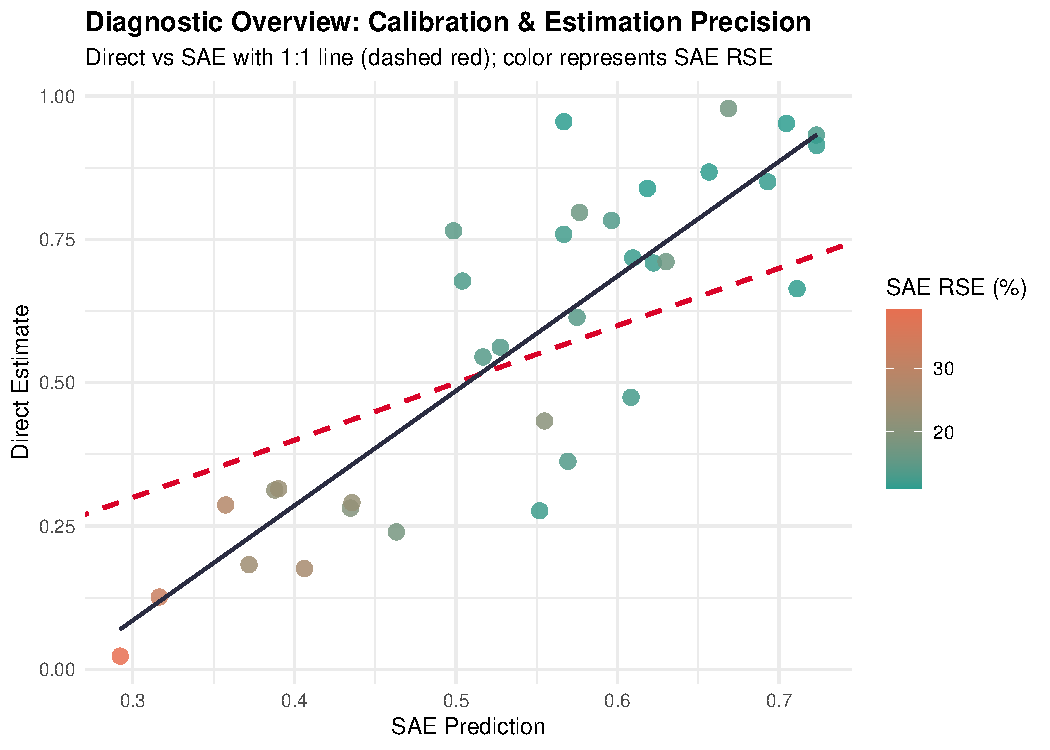
\includegraphics{article-plot_diagnostics}
\caption{\label{fig:diag_plot} Model diagnostic panels produced by \code{autoplot()}.}
\end{figure}

%% -- Summary and Discussion ---------------------------------------------------

\section{Summary and discussion} \label{sec:summary}

In this paper, we introduced \pkg{fastsae}, an \proglang{R} package specifically engineered to resolve the twin challenges of computational intensity and distributional inflexibility in small area estimation. By unifying a compiled \proglang{C++17} linear algebra core with the deterministic Bayesian approximation capabilities of \pkg{R-INLA}, \pkg{fastsae} equips researchers and official statisticians with a fast, versatile, and scalable computational framework. 

The package provides significant practical advantages over existing software:
%
\begin{itemize}
  \item \textbf{Performance}: Multi-threaded OpenMP execution accelerates classical and spatial EBLUP bootstrap MSE estimation by an order of magnitude compared to interpreted \proglang{R} routines in \pkg{sae}.
  \item \textbf{Distributional Scope}: Bayesian EBP via INLA seamlessly accommodates six likelihood families (Gaussian, Beta, Gamma, Binomial, Poisson, Negative Binomial) with exact design variance preservation via \citet{janicki2020properties} dispersion matching and Gamma CV scaling.
  \item \textbf{Modern Spatial Prioirs}: Graph-based random effects---including BYM, scaled BYM2 with Penalized Complexity priors, and Leroux CAR with exact structure matrix formulation ($C = I - R$)---can be specified through a single intuitive argument.
  \item \textbf{Production Readiness}: Automatic handling of unsampled domains, integrated leave-one-out predictive diagnostics (CPO/PIT), and \pkg{ggplot2} visual summaries make the package ideally suited for automated publication pipelines in national statistical agencies.
\end{itemize}

Future developments include extending \code{ebp\_area()} to zero-inflated Beta (ZIB) likelihoods for sparse demographic indicators, supporting spatio-temporal INLA formulations with type I--IV space-time interactions, and integrating direct spatial polygon shapefile inputs.

%% -- Computational Details & Acknowledgments ----------------------------------

\section*{Computational details}

The results in this paper were obtained using \proglang{R}~4.4.2 with the packages \pkg{fastsae}~0.1.0, \pkg{R-INLA}~24.06.27, \pkg{sae}~1.3, \pkg{emdi}~2.2.1, \pkg{tipsae}~1.0.1, and \pkg{ggplot2}~3.5.1. \proglang{R} itself and packages from CRAN are available at \url{https://CRAN.R-project.org/}. \pkg{R-INLA} is available from \url{https://www.r-inla.org/}. The \pkg{fastsae} package is available on GitHub at \url{https://github.com/ridsonap/fastsae}.

\section*{Acknowledgments}

The authors thank the Department of Computational Statistics and Department of Statistics at Politeknik Statistika STIS for institutional support. We also acknowledge the feedback and domain expertise provided by colleagues at BPS-Statistics Indonesia.

%% -- Bibliography -------------------------------------------------------------

\bibliography{refs}

\end{document}
